\subsection{Numerical accuracy}\label{sec:val-numerics}

The likelihood of Section~\ref{sec:likelihood} is a deterministic numerical solution, so its accuracy can be measured
against references that do not share its code. All results below are from stored acceptance runs of the current engine
unless marked as the previous solver. Table~\ref{tab:numerics} lists them; the paragraphs give the sub-quantities,
including those that failed.

\begin{table}[t]
\centering\small
\caption{Numerical checks of the current engine. Each row asks one question about the likelihood; the reference is
computed independently of the engine's code. ``Status'' is the verdict written to the stored result file: a file is
marked ``fail'' when any of its sub-checks fails, even if the main result passes. The failures are listed in the last
column and discussed in the text.}\label{tab:numerics}
\begin{tabular}{@{}>{\raggedright\arraybackslash}p{4.4cm}>{\raggedright\arraybackslash}p{3.2cm}>{\raggedright\arraybackslash}p{3.6cm}>{\raggedright\arraybackslash}p{3.6cm}@{}}
\toprule
What is checked & Reference & Main result & Status and failures\\\midrule
\emph{Same numbers as an independent implementation?} The log-likelihood, each of its terms, survival and gradient,
  compared one evaluation at a time.
  & a separate NumPy implementation of the same equations, \C{acc-t1-evals} evaluations
  & worst total error \C{acc-t1-library-nonSweden-total-s} nats (all cohorts but the largest)
  & fail: \C{acc-t1-fail} evaluations (round-off on the largest cohort; a finite-difference gradient check)\\[2pt]
\emph{Unlikely deaths scored accurately?} Deaths that the model makes very improbable decide whether a likelihood can
  be used far from the optimum; their probabilities are tiny differences that lose digits easily.
  & the same scheme in \C{acc-mp-dps}-digit arithmetic, \C{acc-mp-neval} evaluations
  & worst error \C{acc-mp-v1-lowmass-s} nats summed over an evaluation's unlikely deaths
  & fail: \C{acc-mp-roundoff-fail} of \C{acc-mp-roundoff-n} evaluations on the largest cohorts (float64 round-off)\\[2pt]
\emph{Early deaths scored accurately?} Early in life the death density changes fastest, so these terms carry the
  largest grid error.
  & a reference converged on successively refined graded meshes
  & \C{acc-early-converged} of \C{acc-early-rows} references converged
  & fail: \C{acc-early-unconv} references did not converge\\[2pt]
\emph{Converges to an exact answer?} With no production and no removal the survival curve is known in closed form.
  & closed-form series
  & observed order \C{acc-anchor-order} in the grid spacing, as expected
  & pass\\[2pt]
\emph{Unbiased at the truth?} At the true parameters the average gradient of the log-likelihood over many simulated
  cohorts must be zero.
  & cohorts simulated from the model
  & largest $|z|$ over all features \C{acc-score-hazard} (with an external hazard), below the threshold \C{acc-score-zcrit}
  & fail: the window and heterogeneity tests could not detect their own planted errors, so they are not informative\\
\bottomrule
\end{tabular}
\end{table}

\paragraph{Independent implementation.} The engine's log-likelihood terms, survival values $S$ and gradients were
compared with the frozen NumPy implementation of the original code on \C{acc-t1-evals} evaluations (library cohorts,
entry, heterogeneity with a window, and piecewise-constant segments; two time-stepping schemes, parameters at the truth
and perturbed). The acceptance limits were \C{acc-t1-thr-total-s} nats for the total, \C{acc-t1-thr-term-s} for each
resolved term, \C{acc-t1-thr-dS-s} for $|\Delta S|$, and a relative \C{acc-t1-thr-grad-s} for the gradient against automatic
differentiation of a fixed-length march. \C{acc-t1-passed} of \C{acc-t1-evals} evaluations passed. Totals agreed to
\C{acc-t1-hetwindow-total-s} nats for heterogeneity with a window and to \C{acc-t1-library-nonSweden-total-s} nats on every evaluation
other than those on the largest cohort; on library cohorts, resolved terms to \C{acc-t1-resolved-term-s} nats, $|\Delta S|$ to \C{acc-t1-dS-s}, and the
gradient to \C{acc-t1-grad-max-s} on all uniform-mesh evaluations. The \C{acc-t1-fail} failures are of two kinds.
Of these, \C{acc-t1-fail-sweden} are on the largest cohort (a very large and stiff human life table with $n=\C{acc-t1-sweden-n}$), where the total
differs by up to \C{acc-t1-sweden-total-s} nats, above the required $10^{-5}$ nats, from float64 round-off in the implicit step.
The other \C{acc-t1-fail-cd} are failures of a finite-difference cross-check of the gradient, not of a value: the totals
agree to better than $10^{-11}$ nats there.

\paragraph{High-precision reference and the absorbed-flux form.} The same discrete scheme was evaluated in mpmath at
\C{acc-mp-dps} digits on \C{acc-mp-neval} evaluations whose rows have low probability, the rows that decide whether a
likelihood is usable. The reason for including them is a change of formula. The probability mass of a death within a
recording interval is the decrease of survival over the interval, a difference of two numbers close to $1$ when the
mass is small; computed that way (the earlier form) it underflows or is round-off. The engine instead computes it as
the increase of the absorbed flux $F$ through the threshold, whose operands are small, and uses the survival
difference only where its operands are the smaller (Section~\ref{sec:likelihood}). Against mpmath the absorbed-flux form is within
\C{acc-mp-v1-lowmass-s} nats summed over any evaluation's low-probability rows, whereas the earlier subtraction was off by
up to \C{acc-mp-v033-lowmass} nats (Figure~\ref{fig:numerics}A). On a panel of \C{acc-mp-roundoff-n} evaluations at stored,
fitted, seed and perturbed parameters of large cohorts, the error of the earlier form reached \C{acc-mp-v033-seed} nats at a
seed point and \C{acc-mp-roundoff-v033-max-s} nats at ten times the fitted $\eta$; at the stored estimate of the
$n=\C{acc-mp-sweden-n}$ cohort the total log-likelihood differed from mpmath by \C{acc-mp-sweden-v1-s} nats for the
absorbed-flux form and by \C{acc-mp-sweden-v033} nats for the earlier one (Figure~\ref{fig:numerics}B). The
panel has \C{acc-mp-roundoff-fail} failures of the $10^{-5}$ nats limit, all from float64 conditioning of the largest cohorts. At three stiff human
truths both forms are \C{acc-mp-truth-fail-min-s} to \C{acc-mp-truth-fail-max-s} nats off; on the $n=\C{acc-t1-sweden-n}$
cohort the absorbed-flux form is \C{acc-mp-sweden-eps15-dl-s} nats off at $1.5\times\eps$ and its spread under $\pm3$-ulp
perturbations of the parameters is \C{acc-mp-sweden-eta15-spread-s} nats at $1.5\times\eta$.

\begin{figure}[t]
\centering
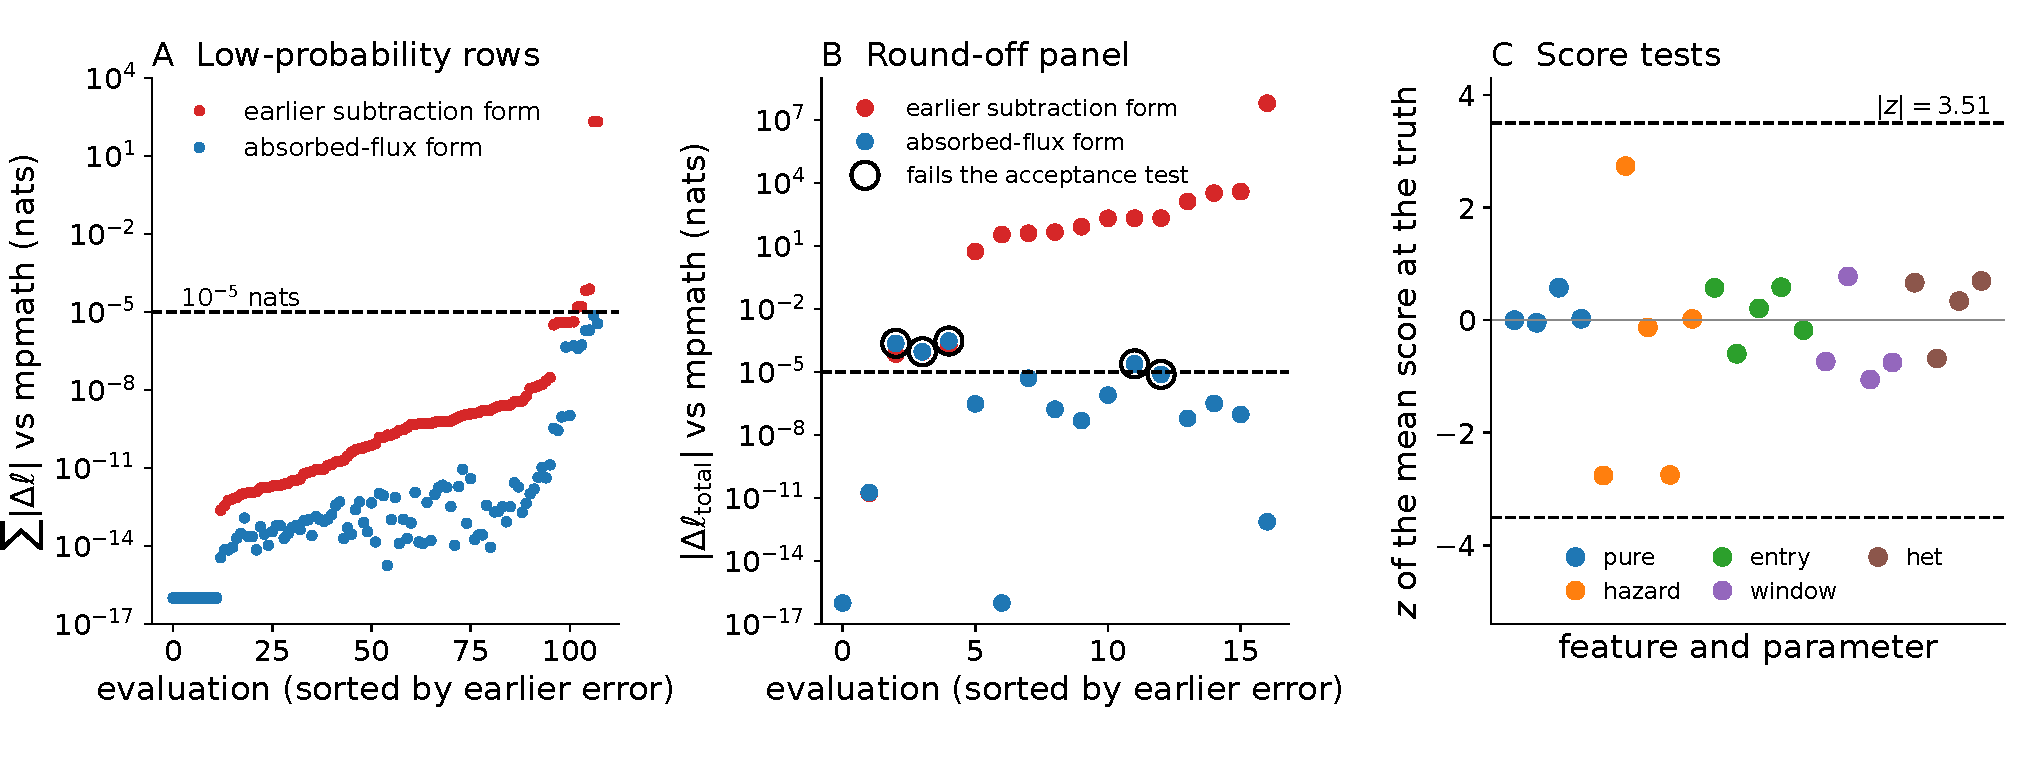
\includegraphics[width=\textwidth]{fig_numerics.pdf}
\caption{Numerical accuracy of the current engine against mpmath and simulation. \textbf{A}, error of the summed
log-probability of the low-probability rows of \C{acc-mp-neval} evaluations, earlier subtraction form and
absorbed-flux form, sorted by the earlier error (values below $10^{-16}$ are drawn at that floor). \textbf{B}, total
log-likelihood error of both forms on the round-off panel, sorted by the earlier error; circles mark the
\C{acc-mp-roundoff-fail} evaluations that fail the $10^{-5}$ nats limit. \textbf{C}, $z$ of the mean score at the true
parameters over simulated cohorts, for each feature and parameter; dashed lines are the multiplicity-corrected
threshold $\pm\C{acc-score-zcrit}$.}\label{fig:numerics}
\end{figure}

\paragraph{Analytic anchor.} For pure diffusion ($\eta=\beta=0$) the survival function has a closed-form series. The
scheme reproduces it at observed order \C{acc-anchor-order} in the grid spacing (the reflecting wall sits half a cell from the start, so
first-order convergence is expected), the maximum $|\Delta S|$ falling from \C{acc-anchor-dS-coarse-s} to \C{acc-anchor-dS-fine-s}
when the grid is refined by a factor of eight, and the errors of early-death terms fall monotonically.

\paragraph{Score tests against simulated cohorts.} At the true parameters the expected score of the exact likelihood
is zero. We simulated \C{acc-score-R-pure} cohorts of $n=\C{acc-score-n}$ from the SR model with the original
Euler/Brownian-bridge simulator (at one eighth of its default time step, because at the default the pure control was
biased by several standard errors), computed the likelihood gradient on each, and tested the mean at a
multiplicity-corrected threshold of $|z|=\C{acc-score-zcrit}$. The largest $|z|$ was \C{acc-score-pure} for the pure
control, \C{acc-score-hazard} with an external hazard (\C{acc-score-R-hazard} cohorts), \C{acc-score-entry} with left truncation
(\C{acc-score-R-entry} cohorts), \C{acc-score-window} for a fit window (\C{acc-score-R-window} cohorts) and \C{acc-score-het} for
heterogeneity in the threshold (\C{acc-score-R-het} cohorts) (Figure~\ref{fig:numerics}C). The scoring file as a whole is marked
``fail'': the window test with \C{acc-score-R-window-big} cohorts and the heterogeneity test did not detect their own planted
alternatives (a deliberately wrong closing rule for the window; node-by-node conditioning for heterogeneity), so their
agreement is not informative at those sample sizes. The window test at \C{acc-score-R-window} cohorts, which did detect its
planted alternative (up to $|z|=\C{acc-score-window-plant}$), passed, and the entry test detected its own. We therefore
have an informative agreement for the pure, hazard, entry and window features and not for heterogeneity.

\paragraph{Early deaths.} Early deaths are the most sensitive terms: of \C{acc-early-rows} early-death terms, \C{acc-early-converged} had a converged graded reference.
The remaining \C{acc-early-unconv} (eight in the $n=\C{acc-mp-sweden-n}$ human cohort, one in a cohort with an added age-0 death) did not
converge; on the former the engine's residuals sum to \C{acc-early-sweden} nats, the largest single term being
\C{acc-early-sweden-max} nats. Grid error is thus a property of the deaths that carry little probability at the fitted
parameters; the software lists them in its fit diagnostics rather than correcting them.% src: sraging docs/algorithms fp_engine.tex, floors phase

\paragraph{Previous solver: Fokker--Planck against Langevin simulation (historical).} Before the current engine, an
earlier Fokker--Planck solver was compared with the Langevin simulation of the original code on all \C{oldsrk-n-presets}
calibrated preset organisms, with \C{oldsrk-npeople} simulated individuals each. The Kolmogorov--Smirnov distance between
the two survival curves was below $0.05$ for \C{oldsrk-ks-below} of \C{oldsrk-n-presets} presets, with a median of \C{oldsrk-ks-median}.
The worst preset had a distance of \C{oldsrk-ks-worst}; the disagreements were on stiff strong-removal presets, and
refining the Langevin time step moved its median lifespan onto the Fokker--Planck value, so they are attributed to the
simulator's step. This is evidence for the previous solver only.

\begin{figure}[t]
\centering
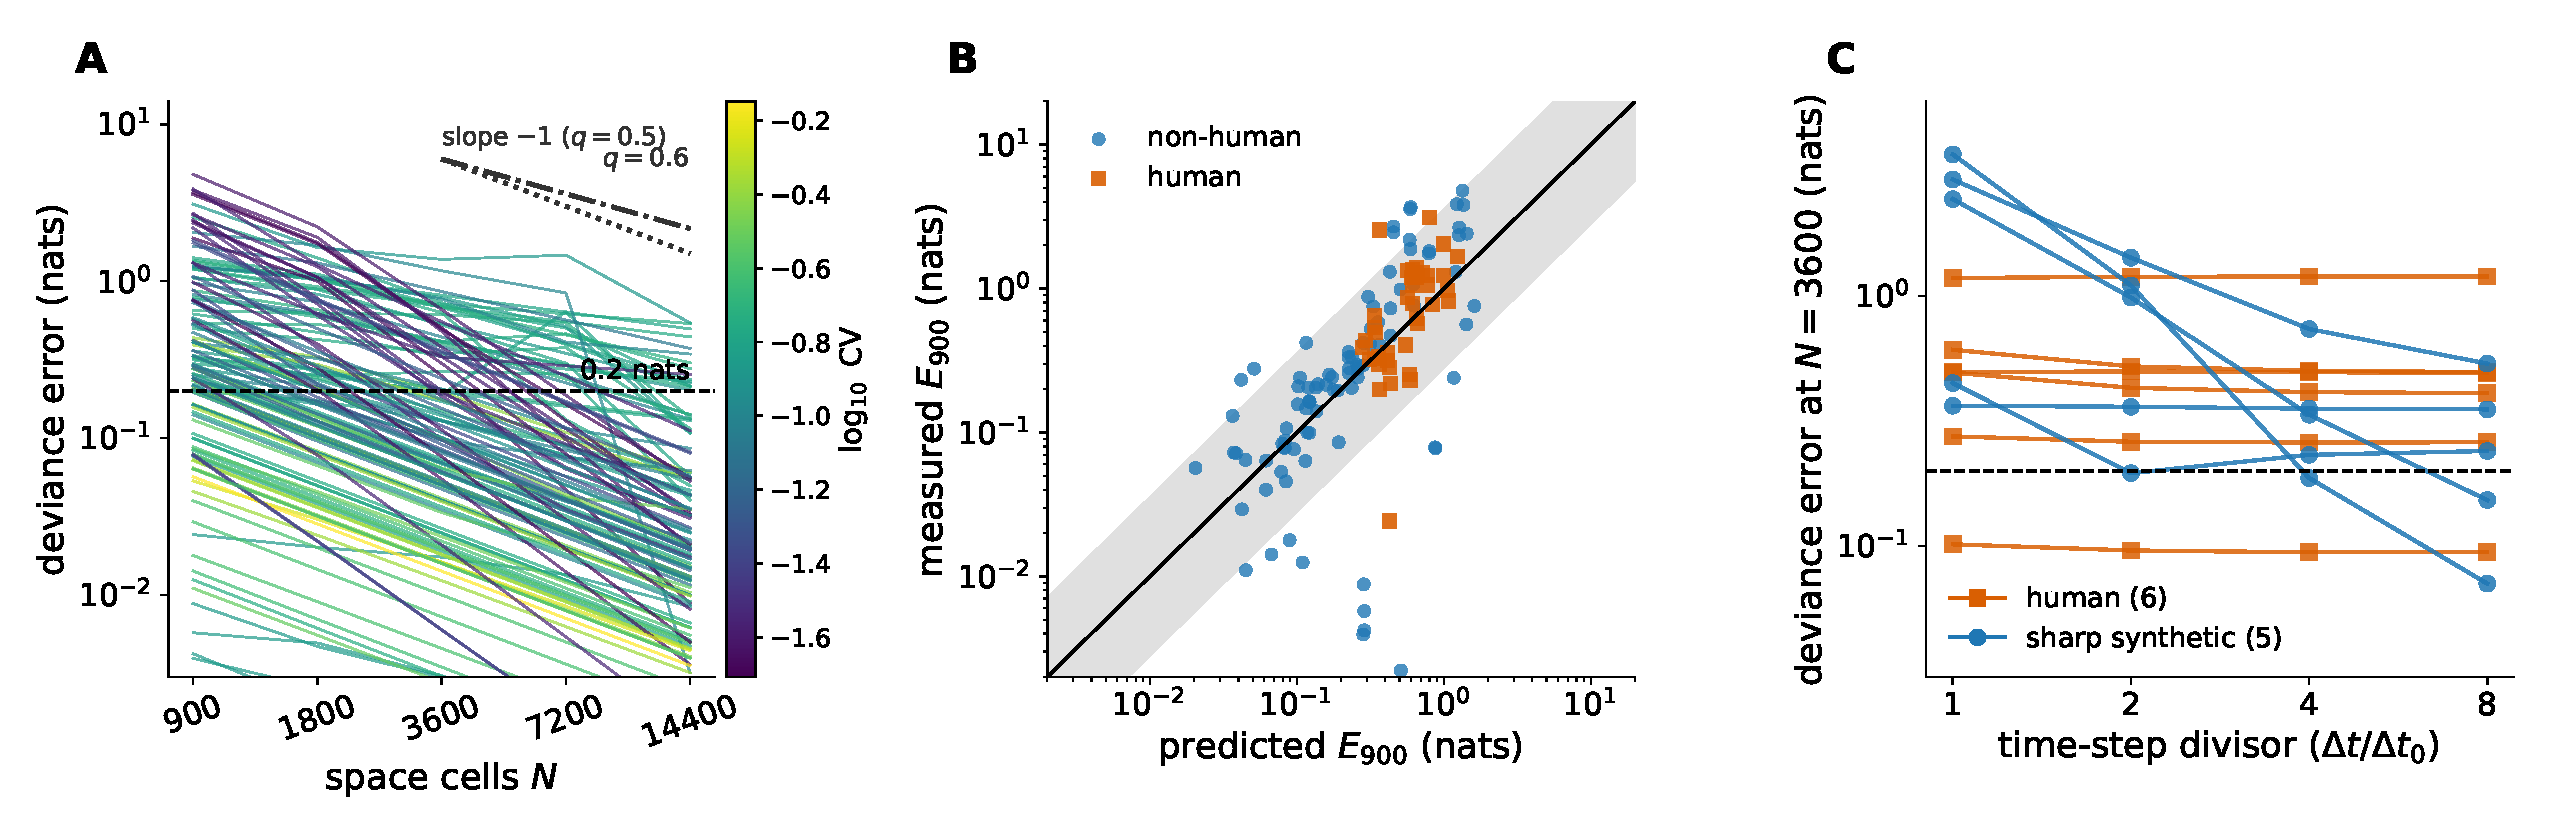
\includegraphics[width=\textwidth]{fig_convergence.pdf}
\caption{Convergence of the log-likelihood deviance with the number of space cells $N$ and the time step, from a stored
grid study of the engine. The deviance is the log-likelihood at a point minus its maximum; the error is the largest
difference, over the points that decide an interval, from a reference limit (see text). \textbf{A}, error against $N$ for each of
the \C{nrule-n} regression cohorts, coloured by the Kaplan--Meier coefficient of variation (CV) of the death age. The dashed line is the
\C{nrule-target}-nat target. The dotted and dash-dotted segments show a contraction by a factor $0.5$ and $\C{m-nr-q}$ per doubling of
$N$. The error at $N=14400$ is partly fixed by the extrapolation that defines the reference. \textbf{B}, measured error at
$N=\C{nrule-N0}$ against the error predicted by the rule from $n$ and CV; the line is equality and the grey band is
$\pm\C{nrule-resid-sd}$ decades, the residual standard deviation of the regression. \textbf{C}, error at $N=3600$ against the
time-step divisor ($1$ is the production step), for the \C{conv-g2-n-h} human cohorts and the \C{conv-g2-n-s} sharp synthetic
cohorts of the joint study; the reference there is the limit at one eighth of the step.}\label{fig:convergence}
\end{figure}

\paragraph{Convergence with grid size and time step.} The grid-rule study measured how the error of the deviance depends on
$N$ and on the time step; every number below is from its stored values. It covers \C{conv-n-measured}
cohorts of the calibration benchmark: \C{conv-n-human-all} human cohorts (library life tables with $n$ up to $10^{5}$, among
them every human cohort on which an earlier interval check failed) and \C{conv-n-nonhuman-all} non-human or synthetic cohorts with
$n$ from \C{conv-n-min} to about $2.5\times10^{4}$. The log-likelihood was evaluated at the points that decide the intervals
(the maximum, the best profile node, and for each parameter and side the two nodes that bracket the
$1.92$-nat crossing, or the outermost node of an unbounded side) on grids of $N=900,1800,\ldots,14400$ cells at the
production step, and at half that step for $N=7200$. The error $E_N$ of a cohort is the largest $|D_N-D_\mathrm{ref}|$ over its
edge points with $|D_\mathrm{ref}|\le\C{conv-edge-cut}$ nats. The reference $D_\mathrm{ref}$ is a Richardson limit
from the three finest grids: with $d$ the last increment of the deviance and $r$ the ratio of the last two increments,
$D_\mathrm{ref}=D_{14400}+d\,r/(1-r)$, accepted only if $0<r<\C{conv-r-max}$; otherwise the finest value is used and the
point is flagged. A second, smaller study crossed $N$ up to $28800$ with the step divided by $1,2,4,8$ on
\C{conv-g2-n} cohorts (\C{conv-g2-n-h} human and \C{conv-g2-n-s} sharp synthetic ones, besides one excluded), with the limit
taken at one eighth of the step.

These cohorts are not a random sample. They were chosen because they were hard: large human cohorts and cohorts where
the benchmark fits had failed or whose intervals were in doubt. The error model was fitted on the \C{nrule-n} of them in
the regime where the numerical value is reproducible (round-off of the log-likelihood at $N=7200$ below
\C{conv-regA-mle} nats at the maximum and \C{conv-regA-best} at the best node; \C{conv-n-regime-a} of the \C{conv-n-measured}
cohorts). The \C{conv-n-reg-human} human and \C{conv-n-reg-nonhuman} non-human cohorts have $n$ from \C{conv-n-min} to
\C{conv-n-max} and CV from \C{conv-cv-min} to \C{conv-cv-max}. The remaining human cohorts have a maximum at the edge of the
parameter box, where refining the grid makes the value noisier, not better; they are not part of the fit, and neither are three
sharp synthetic cohorts whose maximum is far from the truth. Shares of cohorts within a tolerance below therefore describe
this difficult set and understate what a typical dataset would reach.

The error falls by about half with each doubling of $N$ (Figure~\ref{fig:convergence}A): the median ratio $E_{2N}/E_N$ is
\C{conv-r-med}, with a third quartile of \C{conv-r-q75} and a ninth decile of \C{conv-r-q90} (pooled over the doublings
from $900$ to $7200$ at which $E_N>0.05$ nats; \C{conv-r-npairs} ratios). The contraction is first order, as for the analytic
anchor above, on non-human cohorts (median \C{conv-r-med-nonhuman}, ninth decile \C{conv-r-q90-nonhuman}) but slower on human
cohorts (median \C{conv-r-med-human}, ninth decile \C{conv-r-q90-human}). The error also depends on the cohort. At $N=\C{nrule-N0}$ the
median is \C{conv-e900-med-human} nats on human and \C{conv-e900-med-nonhuman} nats on non-human cohorts. For the
\C{conv-n-h1e5} human cohorts with $n=10^{5}$ the median error is \C{conv-h1e5-e900} nats at $N=\C{nrule-N0}$, \C{conv-h1e5-e3600} at
$N=\C{nrule-cap}$ and \C{conv-h1e5-e14400} at $N=14400$.

The time step matters for sharp cohorts and little otherwise. Halving the step at $N=7200$ moves the deviance by a median of
\C{conv-dt-h-med} nats on human cohorts but by \C{conv-dt-sharp-med} nats on the \C{conv-n-sharp} cohorts with CV below $0.05$. In the joint
study the median error of the sharp cohorts at $N=\C{nrule-cap}$ falls from \C{conv-g2-s-dt1} nats at the production step to \C{conv-g2-s-dt8} nats
at one eighth of it, whereas for human cohorts the step changes the error by at most \C{conv-g2-h-dteffect} nats
(Figure~\ref{fig:convergence}C). Refining $N$ alone does not help a sharp cohort once the time error dominates, which is the reason for
the step rule of Section~\ref{sec:likelihood}.

\emph{What a user can read off.} Compute the Kaplan--Meier CV of the death age and take $n$ as the number of individuals
given to the likelihood. The rule predicts the error at $N=\C{nrule-N0}$ as
$E_{900}=10^{\C{nrule-A}}\,n^{\C{nrule-B}}\,\mathrm{CV}^{\C{nrule-C}}$ nats and at $N=\C{nrule-N0}\cdot2^{k}$ as
$E_{900}\,q^{k}$ with $q=\C{m-nr-q}$. For $n=1000$ and CV $0.2$ the prediction is \C{conv-ex-a-pred} nats, so the production grid
suffices. For $n=10^{4}$ and CV $0.1$ it is \C{conv-ex-b-pred} nats at $N=\C{nrule-N0}$ and \C{conv-ex-b-rule} at the
$N=\C{nrule-cap}$ the rule then uses. For $n=10^{5}$ and CV $0.15$ it is \C{conv-ex-c-pred} nats, and \C{conv-ex-c-rule} at the cap; for human
cohorts of this size the measured median at the cap is \C{conv-h1e5-e3600} nats (above), because their contraction is slower than $q$. The
prediction is a median with a spread: the regression residual has a standard deviation of \C{nrule-resid-sd} decades
(a factor of \C{conv-resid-factor}), the measured error was within a factor of ten of the prediction for \C{conv-resid-within10}\% of the
cohorts, and above it for \C{conv-resid-pos}\%. The ninth decile of the residual is \C{conv-resid-q90} decades above the prediction.

\emph{Effect of the rule.} At the grid the rule chooses, \C{nrule-share-after} of the \C{nrule-n} cohorts are within \C{nrule-target}
nats (\C{nrule-share-before} at $N=\C{nrule-N0}$) and \C{conv-n-erule-le05} within $0.5$ nats (\C{conv-n-e900-le05} at
$N=\C{nrule-N0}$); the median error falls from \C{nrule-med-before} to \C{nrule-med-after} nats, at \C{nrule-cpu-x} times the CPU time. For non-human cohorts \C{conv-n-nh-erule-le02} of
\C{conv-n-reg-nonhuman} reach the target (\C{conv-n-nh-e900-le02} before); for human cohorts only \C{conv-n-h-erule-le02} of \C{conv-n-reg-human}
(\C{conv-n-h-e900-le02} before), with a median error of \C{conv-h-erule-med} nats and a maximum of \C{conv-h-erule-max}. The cap and the rule's
$q$ both limit them; a human cohort of $n=10^{5}$ needs $N=14400$, which float64 conditioning does not allow.

\emph{Engine version.} The study measured the engine as it stood on 3 October 2026, at the commit that introduced the $N$ rule,
using the grids and step stored in the benchmark records (step rule off). The handoff of version 1.0.1 lists the same rule
constants and cap and states that the grid is a function of the data and these constants only; it also records that version 1.0.1 with its
new switches off reproduces 1.0.0 exactly. It does not re-measure grid error, and it adds the graded early mesh and the scoped step rule, which this study
did not test. The figures above are therefore measurements of the earlier engine, applied to 1.0.1 through the unchanged rule.

\paragraph{Current engine: Fokker--Planck against Langevin simulation.} The same comparison was repeated for the current
engine with the current Langevin sampler. For each cell, \C{lgks-n} death times were simulated and the Kolmogorov--Smirnov
distance $D$ to the engine's survival curve was computed. The cells cover the four calibrated presets (mouse, dog,
\emph{E.~coli}, human), a spread of $\mathrm{CV}=0.1$, $0.2$ and $0.3$ in each of $\eta$, $\beta$, $\varepsilon$, $\kappa$ and $\xc$ where the
preset allows it, and the homogeneous case, with the simulator's lower wall either clamped at zero or reflected. This gives
\C{lgks-n-clamp} clamp cells and \C{lgks-n-reflect} reflect cells (\C{lgks-ncell-mouse} for the mouse, \C{lgks-ncell-dog}
for the dog, \C{lgks-ncell-ecoli} for \emph{E.~coli}, \C{lgks-ncell-human} for the human; the \emph{E.~coli} clamp rows are
left out, see below). A cell passes if $D$ is below the 5\% point of the Kolmogorov distribution divided by $\sqrt n$, with
the level split across the cells of its wall (Bonferroni): $D<\C{lgks-crit-clamp}$ for clamp and $D<\C{lgks-crit-reflect}$ for
reflect. Each cell is run once, at a Langevin time step fixed beforehand from a convergence ladder so that the step's own
bias is at most a tenth of the threshold. All \C{lgks-ncells-all} cells passed (Figure~\ref{fig:langevin}). The largest $D$ was
\C{lgks-maxD-mouse} for the mouse, \C{lgks-maxD-dog} for the dog, \C{lgks-maxD-ecoli} for \emph{E.~coli} and \C{lgks-maxD-human} for
the human, and no cell exceeded \C{lgks-maxratio} of its threshold.

A pass is informative only if the test could have failed, so each wall's family contains a planted error. In two cells
(the dog, homogeneous; the mouse, spread in $\xc$) the Langevin sample was drawn with $\eta$ increased by
\C{lgks-plant-delta-dog}\% and \C{lgks-plant-delta-mouse}\% respectively, a shift sized beforehand to be detectable at this $n$. Both
were rejected, at $D=\C{lgks-plant-D-dog}$ and $\C{lgks-plant-D-mouse}$, about three times the threshold. A second
family of checks, for mixtures over two to three heterogeneous parameters, gives the same picture: all \C{lgks-multi-n}
cells passed (largest $D=\C{lgks-multi-maxD}$ against $\C{lgks-multi-crit}$) and all \C{lgks-multi-plants} planted
errors were rejected ($D\ge\C{lgks-multi-plant-minD}$). The first run of this family failed one cell by a small margin
($D=\C{lgks-multi-first-D}$); it was diagnosed as chance (the step bias and the reference were ruled out), and the
second run, with fresh random numbers and the rule declared beforehand, is the one that passed; both are stored. Simulated
\emph{paths} (not only death times) agree with the engine at \C{lgks-paths-clamp} clamp and \C{lgks-paths-reflect} reflect
test ages.

Three results are not passes. (i) The clamp does not agree with the engine for \emph{E.~coli} at any affordable step: the step
ladder was run up to $m=\C{lgks-pp-ecoli-m}$ substeps and the pooled step bias was still $\C{lgks-pp-ecoli-D}$ against a bar of
$\C{lgks-pp-ecoli-bar}$, so the \emph{E.~coli} clamp rows are excluded from the clamp family and only its reflect rows are
tested. (ii) The step-size study that fixes these steps was stopped by its CPU cap, at \C{lgks-pp-spent} CPU-hours against a cap of
\C{lgks-pp-cap}, after \C{lgks-pp-ran} of its \C{lgks-pp-planned} cells; its status is ``capped''. (iii) A separate test,
that the mean score of the Langevin sample is zero at the truth, is recorded as ``\C{lgks-s5-status}'': \C{lgks-s5-npass} of its
\C{lgks-s5-nfeat} features pass, and the heterogeneity feature is not informative at \C{lgks-s5-R} cohorts of
\C{lgks-s5-n} individuals, as for the earlier score tests above. This is a test of the likelihood gradient rather than of the
survival curve, so it does not affect the comparison reported here. All of this concerns the simulator's
agreement with the engine on the presets; it says nothing about cohorts far from them.

\begin{figure}[t]
\centering
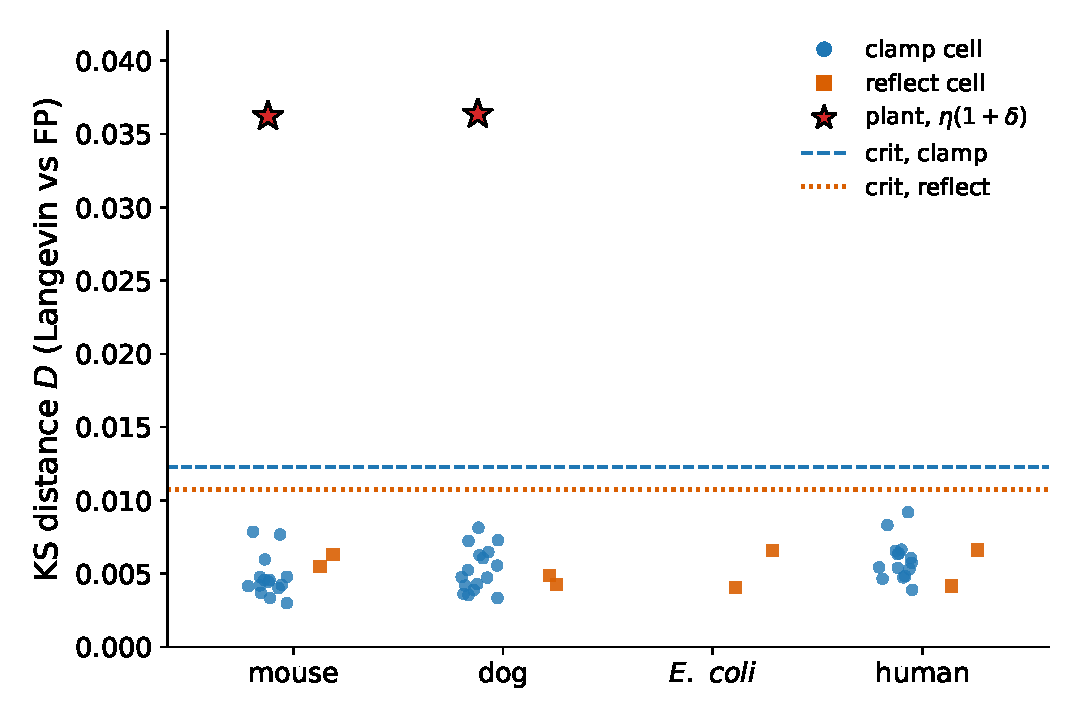
\includegraphics[width=0.55\linewidth]{fig_langevin.pdf}
\caption{Kolmogorov--Smirnov distance $D$ between \C{lgks-n} Langevin death times and the engine's survival curve, one point
per cell, grouped by preset. Blue circles: clamped wall (\C{lgks-n-clamp} cells); orange squares: reflecting wall
(\C{lgks-n-reflect} cells). Dashed and dotted lines: the pass thresholds ($\C{lgks-crit-clamp}$ and $\C{lgks-crit-reflect}$). Stars:
cells in which $\eta$ was deliberately shifted by \C{lgks-plant-delta-dog}\% (dog) and \C{lgks-plant-delta-mouse}\% (mouse); these
are meant to be rejected and are. The \emph{E.~coli} clamp rows are not tested.}\label{fig:langevin}
\end{figure}
